\documentclass{beamer}
\usepackage[utf8]{inputenc}
\usepackage[T1]{fontenc}

\title{Project Report}
\subtitle{\textit{Week 4}}
\date[]{2024/2025}
\author[Fritz]{Fritz Adelbertus Sitindaon}

\usetheme{Warsaw}
\setbeamertemplate{footline}[frame number]
% ===== Setup Font =====
\usepackage[sfdefault,lf]{carlito}
\usepackage[T1]{fontenc}
\renewcommand*\oldstylenums[1]{\carlitoOsF #1}

% ==== Import Math Packages =====
\usepackage{amsmath, amssymb, amsthm}
\usepackage{mathtools}

% ==== There required =====
\usepackage[dvipsnames]{xcolor}
\usepackage[most]{tcolorbox}
\def\wallpaper{wallpaper.jpg}

\def\R{\mathbb{R}}
\def\P{\mathbb{P}}
\def\N{\mathbb{N}}
\def\O{\mathbb{O}}


\def\nX{\mathcal{X}}
\def\nY{\mathcal{Y}}
\def\nT{\mathcal{T}}
\def\nU{\mathcal{U}}
\def\nB{\mathcal{B}}
\def\nS{\mathcal{S}}
\def\nP{\mathcal{P}}
\def\nA{\mathcal{A}}
\def\nF{\mathcal{F}}
\newcommand{\comp}[1]{\overline{#1}} 

\DeclarePairedDelimiter\abs{\lvert}{\rvert}
\DeclarePairedDelimiter\floor{\lfloor}{\rfloor}
\DeclarePairedDelimiter\cic{[ }{] }
\DeclarePairedDelimiter\oic{( }{] }
\DeclarePairedDelimiter\cio{[ }{) }
\DeclarePairedDelimiter\oio{( }{) }
\DeclarePairedDelimiter\set{\{ }{\} }
\DeclarePairedDelimiter\brk{(}{)}
\DeclarePairedDelimiter\seq{\langle}{\rangle}

\begin{document}

\begin{frame}
\titlepage
\end{frame}



\begin{frame}{Revisi dari Minggu Sebelumnya}
    Problem minggu sebelumnya: Output yang keluar 0.0 pada setial sel grid
    \\Alasan:
    \begin{enumerate}
        \item Kesalahan di input
        \item Kesalahan di rumus yang diimplementasi
    \end{enumerate}
    Progres: Output sudah sesuai
\end{frame}

\begin{frame}{Fitur Tambahan}
    Beberapa fitur yang ditambahkan pada minggu ini:
    \begin{enumerate}
        \item Output sudah ada dalam file (namun belum dalam bentuk/format output yang sesuai)
        \item Gelombang awal bisa diperoleh dari file input (tidak harus dari input patahan)
    \end{enumerate}
\end{frame}

\begin{frame}{Refactor and FP Concept Application}
    Beberapa konsep FP yang diterapkan minggu ini:
    \begin{enumerate}
        \item Higher Order Function Application
        \item Point-Free Style
        \item Function Compositions 
    \end{enumerate}
\end{frame}

\begin{frame}{Refactor and FP Concept Application}
    Higher Order Function Application
    \begin{center}
        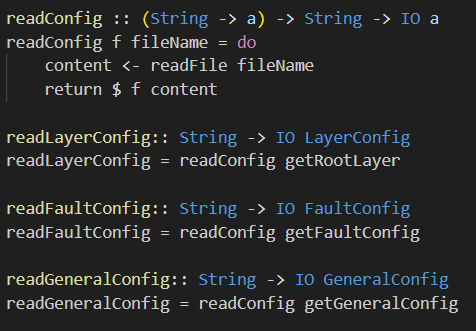
\includegraphics[scale=0.7]{figure/composition.png}
    \end{center}
\end{frame}

\begin{frame}{Refactor and FP Concept Application}
    Point-Free Style and Function Compositions
    \begin{center}
        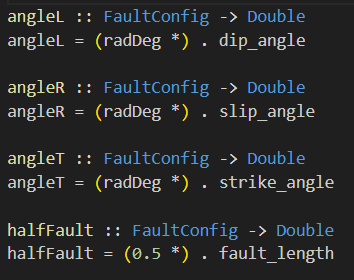
\includegraphics[scale=1.0]{figure/highorder.png}
    \end{center}
\end{frame}

\begin{frame}{Analisa Perbandingan Fortran dan Haskell}
    Memory Usage:\\
    Input yang digunakan adalah grid berukuran 300x400
    \begin{enumerate}
        \item Fortran, RAM yang digunakan tidak melebihi 4000 MB
        \item Haskell, RAM yang digunakan melebihi 8000 MB
    \end{enumerate}
\end{frame}

\begin{frame}{Analisa Perbandingan Fortran dan Haskell}
    Speed:\\
    Input yang digunakan adalah grid berukuran 300x400
    \begin{enumerate}
        \item Fortran, Untuk memperoleh file output pertama diperlukan waktu $\leq 2$ menit
        \item Haskell, Untuk memperoleh file output pertama diperlukan waktu $\geq 7$ menit
    \end{enumerate}
\end{frame}


\begin{frame}{Analisa Perbandingan Fortran dan Haskell}
    Beberapa alasan penyebab performa ini:
    \begin{enumerate}
        \item Fortran memiliki fitur alokasi memori yang efisien dalam komputasi numerik
        \item Perhitungan numerik yang efisien juga mengjadi kelebihan yang diutamakan Fortran
        \item Haskell \textit{by default} menerapkan lazy evaluation yang kurang cocok dalam
        tahap manipulasi grid
    \end{enumerate}
\end{frame}

\begin{frame}{Kelebihan Haskell dalam project ini}
    Beberapa kelebihan haskell yang ada pada program ini:
    \begin{enumerate}
        \item Code Readability, kode dalam haskell lebih mudah untuk dipahami 
        dan disesuaikan dengan Manual COMCOT, alur program juga lebih jelas dibanding
        Fortran
        \item Mathematical Abstraction, penerapan rumus matematika kedalam kode tidak
        memerlukan banyak modifikasi dari penjelasan di Manual COMCOT.
    \end{enumerate}
\end{frame}

\begin{frame}{Kesimpulan}
    Usage:
    \begin{enumerate}
        \item For practical usage in research using COMCOT model, use Fortran.
        \item For academic studies on understanding how the model works, and how it is
        programed, use Haskell
    \end{enumerate}
    Users:
    \begin{enumerate}
        \item Fortran, for general users of the program
        \item Haskell, for academic people who want to understand the model
    \end{enumerate}
\end{frame}

\begin{frame}{Porting Report}
    Fortran Code: 2202 lines read\\
    Haskel Code: 1118 lines writed
\end{frame}

\begin{frame}{Next Week Target}
    Target for Next Week:
    \begin{enumerate}
        \item Finishing the output to precisely mimic the output in COMCOT Fortran
        \item Adding comments and reorienting the order of functions in code for 
        better readability and easier though process when reading
        \item Creating a documentation/README
    \end{enumerate}
\end{frame}
\end{document}